\documentclass[10pt]{article}

\usepackage[a4paper,margin=24mm]{geometry}
\usepackage[T1]{fontenc}
\usepackage{lmodern}
\usepackage{amssymb}
\usepackage{amsmath}
\usepackage{booktabs}
\usepackage{graphicx}
\usepackage{microtype}
\usepackage{xcolor}
\usepackage{hyperref}
\usepackage{url}

\hypersetup{
  colorlinks=true,
  linkcolor=blue!55!black,
  citecolor=blue!55!black,
  urlcolor=blue!55!black,
  pdftitle={DA3-CAD: Deterministic Multi-View RGB-to-B-Rep Reconstruction with Depth Anything 3},
  pdfauthor={DA3-CAD Contributors},
  pdfkeywords={photo-to-CAD, multi-view reconstruction, B-Rep, Depth Anything 3, CAD grammar}
}
\newcommand{\system}{DA3-CAD}
\newcommand{\da}{DA3-LARGE-1.1}

\title{\system: Deterministic Multi-View RGB-to-B-Rep Reconstruction\\with Depth Anything 3}
\author{DA3-CAD Contributors\\\small Author list and affiliations to be finalized before submission}
\date{Working manuscript, 13 August 2026}

\begin{document}
\maketitle

\begin{abstract}
Image-based 3D reconstruction can recover depth, cameras, and visible surfaces,
but these outputs are not an editable boundary-representation (B-Rep) CAD
program.  We present \system, an open pipeline that converts object-centric
multi-view RGB or moving-camera video into executable CadQuery, STEP, and STL.
Depth Anything 3 (DA3) supplies depth, confidence, intrinsics, and extrinsics.
Before DA3 inference, a user or robot explicitly identifies the target instance
with per-view boxes or masks.  Pinned SAM2 converts boxes to masks and a
shared-shape crop retains projective scale and scene context.  The deterministic
geometry stack keeps raw profile evidence separate from a filtered surface cloud
and invokes a class-free CAD grammar.  Extrusion recovers an arbitrary line loop
or circle and admits circular cuts only when mask topology and a matching raw 3D
void agree.  Revolution first tests measured radial evidence, then admits an
outer silhouette-derived axial profile only under strict multi-view stability
gates.  Unsupported geometry is rejected rather than forced into a part
template.  On
three calibrated eight-view fixtures, the same grammar yields valid STEP for a
block, flange, and L-bracket with 87.99\%, 91.82\%, and 89.24\% reference mesh
IoU.  Four masks confirm the flange cut while raw 3D measures its diameter as
10.83\,mm versus 12.00\,mm reference; the L-profile needs no L class.  A licensed
five-video Objectron gate processes 200 target-prepared images in five
40-frame pools.  Adaptive pose selection sends 183 images to reconstruction.
Two runs emit kernel-valid STEP, but the coverage/surface-provenance gate
accepts only the book; bottle remains unsafe, while camera, handled-cup, and
open-laptop explicitly abstain.  Since these real cases have neither reference CAD
nor physical scale, they support integration and failure claims, not dimensional
accuracy.  The system records hypothesis boundaries, scale evidence,
source/model hashes, and independent reference-CAD metrics.  We position it as
a reproducible step from visible geometry to a compositional CAD grammar.
\end{abstract}

\noindent\textbf{Keywords:} photo-to-CAD, multi-view reconstruction, B-Rep,
Depth Anything 3, CAD grammar, reproducibility

\section{Introduction}

A useful answer to ``is 3D reconstruction solved?'' depends on the requested
output.  Structure from motion can estimate cameras and sparse geometry;
multi-view depth can recover dense visible surfaces; neural rendering can
reproduce novel views; and meshing can produce a watertight triangle surface.
Engineering CAD requires additional commitments: analytic or parametric
features, topology accepted by a CAD kernel, physical units, editable
constraints, and ideally the construction logic intended by a designer.  A
visually plausible surface may therefore be an invalid solid, while a valid
solid may contain the wrong hole, thickness, or hidden cavity.

Depth Anything 3 (DA3) predicts spatially consistent geometry from arbitrary
visual inputs with or without supplied camera poses\cite{lin2025depthanything3}.
Its public API exposes depth, confidence, intrinsics, and extrinsics, making it
a strong observation model for a photo-to-CAD system.  DA3 does not itself
claim to emit STEP or design history.  \system{} explores a deliberately simple
and inspectable bridge from these geometric observations to a coarse B-Rep.

The contributions of this working system are:
\begin{enumerate}
  \item an end-to-end, deterministic path from ordered RGB views or video to a
        validated single-solid CadQuery/STEP/STL output;
  \item explicit camera, foreground, coordinate, scale, and failure contracts
        around a pinned DA3 model and source revision;
  \item a class-free construction grammar that recovers line/circle sketches,
        dual-evidence circular cuts, axial revolution profiles, and visible
        open-ended inner profiles without learned CAD-generator weights;
  \item a full-pool DA3 pose pass, adaptive mask/view selection, and a fresh
        selected-subset depth pass that records exhausted capture coverage;
  \item input-evidence selection between extrusion and revolution, with explicit
        abstention when neither operation explains the observations;
  \item restricted execution and independent reference-mesh evaluation, with
        input consistency kept separate from ground-truth accuracy; and
  \item reproducible calibrated fixtures that expose both success and residual
        contour/feature error.
\end{enumerate}

The method is not presented as universal reverse engineering.  Its role is to
establish a transparent baseline on which learned feature recognition and
constraint solving can be evaluated.

\section{Related Work}

\paragraph{Any-view geometry.}
DA3 uses a unified depth--ray formulation for monocular, multi-view, and
pose-conditioned geometry\cite{lin2025depthanything3}.  \system{} consumes the
released prediction contract rather than modifying its network.  When video
poses are available, we recover them with incremental structure from motion in
COLMAP\cite{schonberger2016sfm} and condition DA3 on those cameras.

\paragraph{Foreground and visible geometry.}
Silhouette and depth evidence constrain only observed geometry; concavities
that affect neither remain ambiguous\cite{laurentini1994visualhull}.
Promptable SAM2 converts a user-selected box to an instance mask
\cite{ravi2024sam2}; exact masks remain accepted.  This separates target
selection from class recognition.  A legacy colour/depth/GrabCut path
\cite{rother2004grabcut} remains only for simple central-object scenes.

\paragraph{Parametric CAD.}
CadQuery provides a Python interface to a parametric OpenCascade-based CAD
kernel and exports STEP in addition to tessellated formats\cite{cadquery}.
Contemporary image-to-CAD research often learns command sequences or implicit
shape priors.  Our baseline instead exposes a deterministic grammar of sketch
primitives and operations.  Its implemented subset supports line/circle outer
loops, dual-evidence circular cuts, extrusion, and gated axial revolution.  It
does not name part classes; unsupported evidence is reported explicitly.  This sacrifices
breadth in exchange for traceable geometry and failure behaviour.

\section{Problem Formulation}

Let $I_i$ denote $N$ RGB observations of one rigid object.  Target prompts
$T_i$ are per-view boxes or masks.  Optional inputs are camera intrinsics $K_i$,
world-to-camera transforms $E_i$, and one named physical dimension $d_j$ in
millimetres.  Target preparation yields masks $M_i$.  The output target is a
program $P(\theta)$ that executes to exactly one positive-volume B-Rep solid,
where $\theta$ contains editable primary dimensions.  The program must export
STEP and STL and be accompanied by provenance $R$.

The reconstruction objective is constrained by visible evidence rather than an
unavailable original feature tree.  In particular, a run without scale evidence
produces a canonical-unit model; a run without reference CAD cannot report CAD
IoU; and a valid program alone is not treated as geometric correctness.

\section{Method}

Figure~\ref{fig:pipeline} illustrates the implemented stages and evidence flow
on the calibrated flange fixture.

\begin{figure}[t]
  \centering
  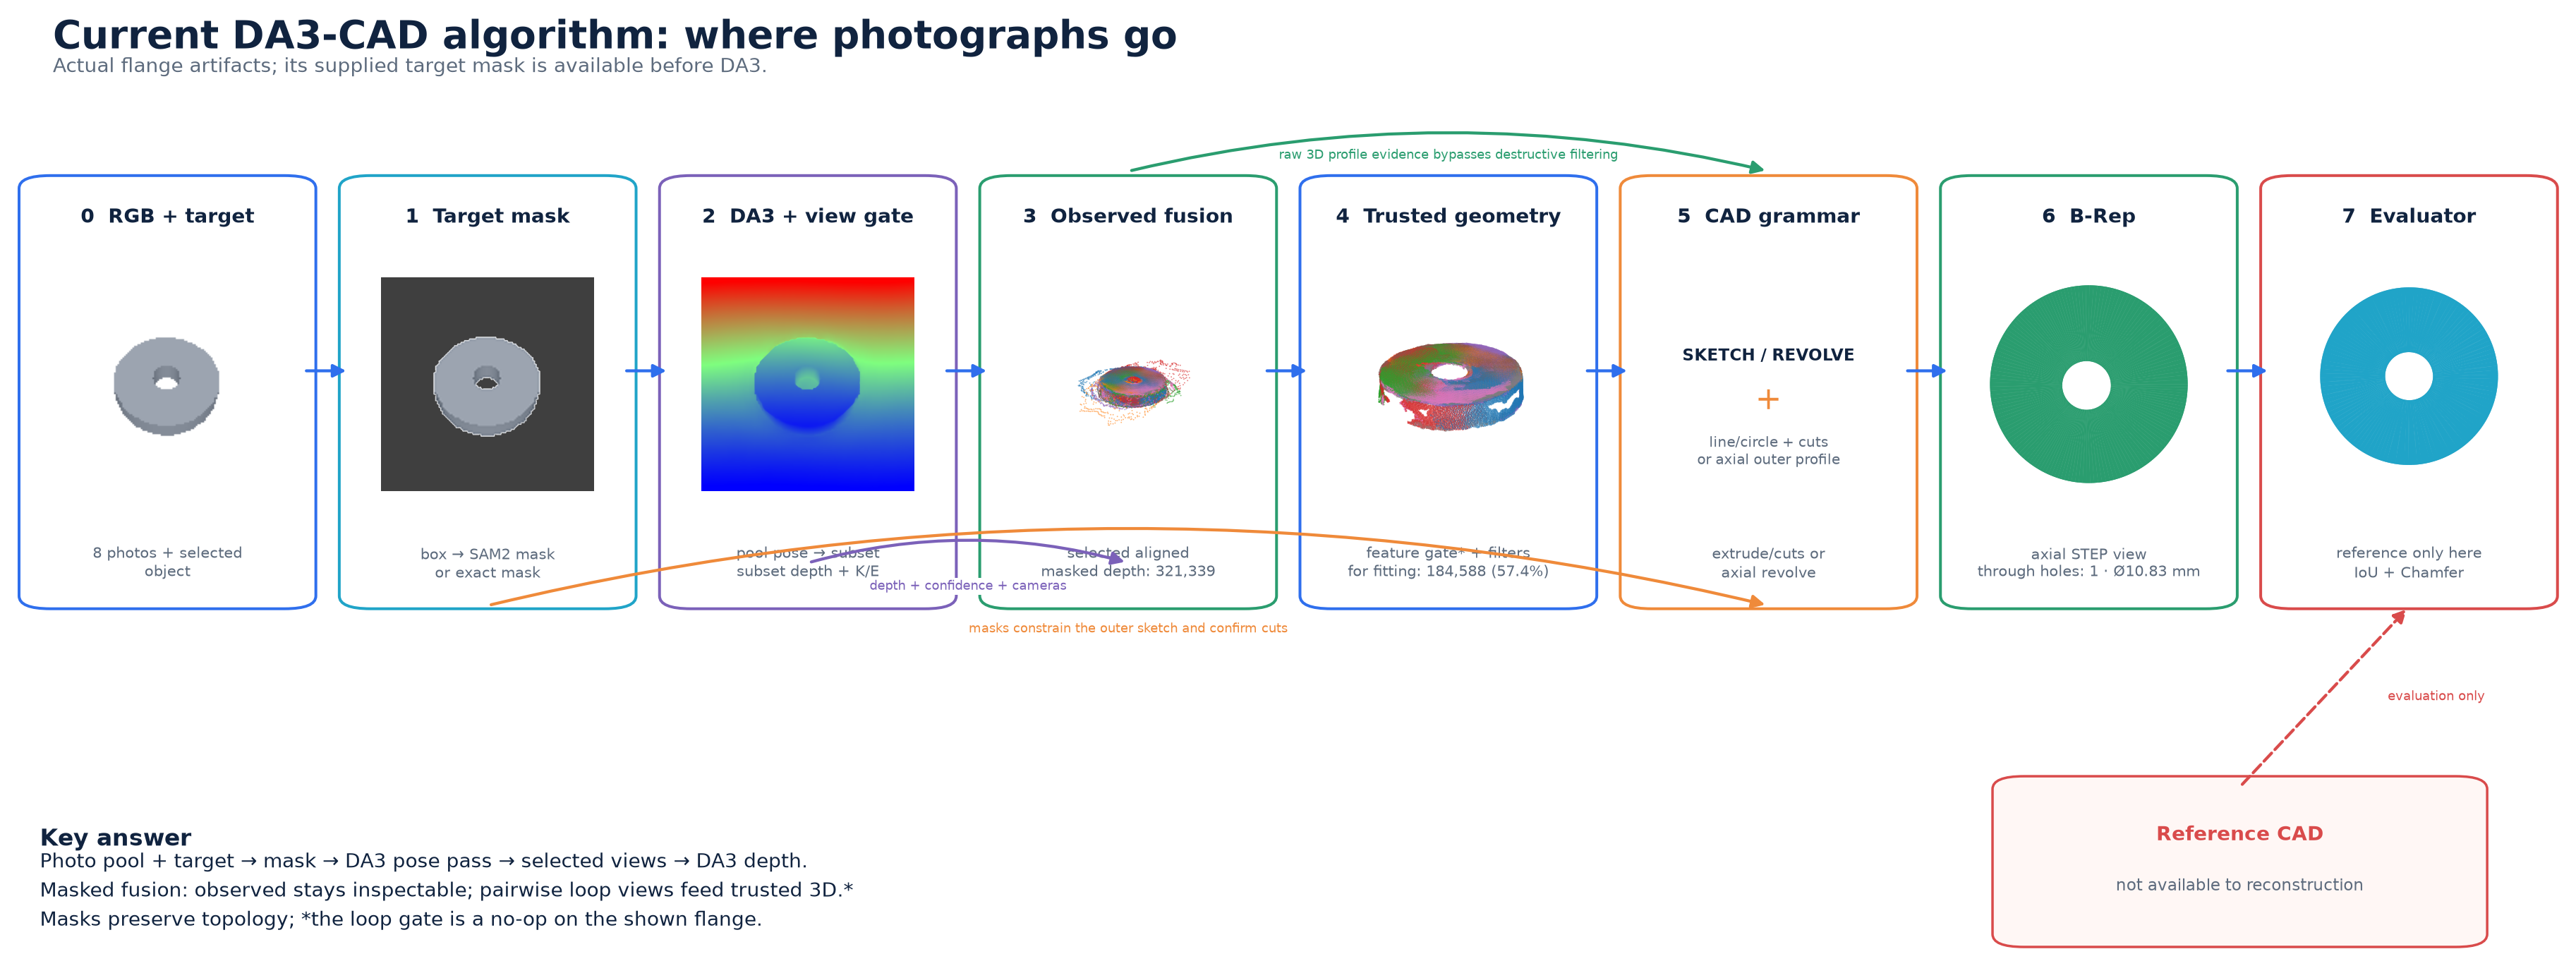
\includegraphics[width=\linewidth]{../docs/assets/benchmark_pipeline/algorithm_flow_en.png}
  \caption{Synthetic supplied-mask path from RGB and DA3 geometry through the
  separate evidence clouds, class-free CAD grammar, and validated B-Rep.}
  \label{fig:pipeline}
\end{figure}

\subsection{Explicit target preparation}

The product path assumes that the operator or robot knows which physical object,
not which part class, it selected.  Each $T_i$ is a loose bounding box or an exact
source-resolution mask.  A pinned SAM2.1 Small predictor converts boxes to masks;
low-score views may add deterministic centre-positive and corner-negative prompts.
Post-processing keeps one box-associated component and preserves enclosed holes
before any DA3 inference.

The sequence is cropped to one shared pixel width and height.  The crop contains
every mask, reduces optional margin before padding, and expands genuine context
until its short-to-long ratio is at least $3:4$.  Individual views are never
resized, so projective scale differences remain observable.  With supplied
cameras, intrinsics are translated by the crop origin while extrinsics remain
unchanged.  The cropped mask is preserved for fusion, hole topology, and grammar
evidence.
\subsection{Pinned DA3 observation model}

We use the official \da{} checkpoint and source at immutable revisions.  The
complete 1.64,GB safetensors file is hashed before every uncached admission.
The adapter validates finite positive depth $D_i$, higher-is-better confidence
$C_i$, $K_i$, $E_i$, and processed images.  Externally supplied cameras
condition DA3 and must survive shape, name, rotation, determinant, and
camera-centre-rank checks.

For a retained pixel $p=[u,v,1]^\top$ with z-depth $z=D_i(u,v)$,
\begin{equation}
  x_{\mathrm{cam}} = zK_i^{-1}p, \qquad
  x_{\mathrm{world}} = E_i^{-1}\begin{bmatrix}x_{\mathrm{cam}}\\1\end{bmatrix}.
\end{equation}
This convention is checked by projection--unprojection round trips at runtime.

\subsection{Masked fusion and separate evidence channels}

The prepared $M_i$ defines object support before unprojection.  The legacy path
may instead derive $M_i$ after DA3 from border colour, central depth, confidence,
GrabCut, morphology, and connected components.  This is retained for simple
central-object images but is not the default real-object evaluation path.

Within $M_i$, every finite positive depth pixel forms the observed channel
$Q_o$.  It is preserved for diagnostics and is not called denoised geometry.  A
separate confidence gate forms trusted fusion $Q_p$; every accepted point keeps
its view and pixel origin.  The product default does not repeat this percentile
gate in canonicalization.  In ablation, two 60th-percentile gates retained only
about 36\% of initially mask-eligible depth points and degraded thin/profile
evidence.  Statistical/radius outlier rejection and minimum neighbourhood
support yield filtered trusted geometry $Q_s$ for orientation and residual
scoring.  The complete $Q_p$ remains profile/aperture evidence, while masks
remain independent boundary/topology evidence.  Filtering is not assumed to be
a monotonic geometric improvement.  No reference shape enters any channel.

\subsection{Adaptive view selection}

For a prepared Internet-video sequence, DA3 first estimates poses for the full
40-frame pool.  Views with near-empty target masks are rejected, then a greedy
selector adds the direction with the largest deterministic spherical-coverage
gain.  It retains at least 24 and at most 40 views and reports
\texttt{sufficient}, \texttt{capped}, or \texttt{exhausted}.  Since DA3 depth
and pose predictions depend on joint batch context, a selected subset is
processed by DA3 again; full-pool depths are never sliced and presented as an
independent reconstruction.  This optimizes acquisition observability, not CAD
accuracy.  The final surface-provenance gate remains authoritative.


\subsection{Camera coverage and CAD-surface provenance}

Recovered camera centres define directions from the robust object centre.  We
cluster near-duplicate directions, report maximum pairwise angle, and estimate
spherical coverage with deterministic sphere samples.  Thus adjacent video
frames do not masquerade as independent opposite views.  When coverage is
insufficient, the report proposes missing camera directions.

After B-Rep construction, deterministic area-weighted CAD surface samples are
projected into every source mask and depth map.  Each sample is labelled
measured, weakly measured, unobserved, or contradicted.  Completion may be
called safe only when camera coverage is insufficient, enough proposed surface
is genuinely unobserved, and visible evidence does not contradict it.  Inferred
surface is never relabelled as measurement.  The current thresholds are an
auditable diagnostic and completion-safety gate, not a calibrated universal CAD
accuracy score.

\subsection{Safe depth hypotheses}

The original DA3 depth is always retained as an identity candidate.  A second
candidate applies one affine depth correction per view using fixed local-plane
agreement across overlapping observations.  The reference view fixes the
gauge.  In automatic mode the aligned candidate is admitted only if the
overlap graph is complete, its robust observation loss decreases by a fixed
margin, all parameters remain within conservative bounds, and the optimizer
does not hit a bound.  This stage accepts only depth, confidence, cameras,
masks, and the deterministic seed; reference CAD is not an API input.

For the implemented sketch-extrusion grammar, both safe candidates are fused
and provisionally fitted.  We retain the candidate with the lower sum of its
normalized P90 distance to the best extrusion surface and a small weighted loss
for raw-profile occupancy erased by sketch simplification, with a stable tie in
favour of identity.  Thus alignment is neither globally enabled nor
globally disabled: it must improve the editable construction that is actually
emitted.

\subsection{Canonical frame and scale}

The system chooses either a three-axis PCA frame or, for planar degeneracy, a
dominant-plane normal plus deterministic in-plane symmetry/PCA voting.  It
records every candidate and tie-break.  Isotropic normalization subtracts the
robust bbox centre and divides all axes by one largest extent; per-axis scaling
is forbidden.

Scale is metadata independent of normalized shape.  If the CAD backend emits a
parameter matching a supplied observation such as
\texttt{extrusion\_length=40mm}, one uniform factor converts every emitted length to
millimetres.  Otherwise scale remains unresolved.  COLMAP units and category
priors are never silently interpreted as physical units.

\subsection{Class-free profile recovery}

Let $Q_s$ be the denoised oriented surface cloud and $Q_p$ the full set of raw
fused observations transformed into the same isotropically normalized frame.
For each candidate extrusion axis $a\in\{x,y,z\}$, the method robustly estimates
end positions $l_a,u_a$ from $Q_s$ and rasterizes the projection of $Q_p$ onto the other two
axes.  It keeps the largest connected component and closes small sampling gaps.
The unfilled raw occupancy remains available for geometric aperture measurement,
while a separately filled copy defines the outer solid: an absent depth sample
alone is not sufficient evidence for a manufactured hole.  The external contour is represented by a
least-squares circle when normalized radial residual is below a fixed threshold;
otherwise it is simplified to a closed line loop.  Raster IoU between that loop
and raw outer-profile occupancy records contour information lost by simplification.

Each axis candidate is scored directly against the three-dimensional evidence.
For point $q$, let $d_s(q)$ be its distance to the extruded profile boundary and
$d_e(q)=\min(|q_a-l_a|,|u_a-q_a|)$ its distance to an end plane.  The surface
residual is
\begin{equation}
  r_a = \operatorname{P90}_{q\in Q_s}\min(d_s(q),d_e(q)) / \operatorname{extent}(Q_s),
  \qquad J_a = r_a + \lambda(1-\operatorname{IoU}_{\mathrm{profile},a}).
\end{equation}
The lowest-cost connected candidate is selected.  If its surface residual exceeds
the fixed limit, the backend returns unsupported rather than choosing a part
class or a nearest primitive.

\subsection{Mask-supported cuts and B-Rep program}

Enclosed background components are extracted independently from each input
mask.  Their contours are ray-lifted to the selected profile end plane using
$K_i,E_i$, fitted as circles, and clustered by centre and radius.  Separately,
enclosed components in the raw 3D-profile occupancy are circle-fitted.  A
circular cut enters the sketch only when a mask cluster repeats in at least two
views and matches a raw 3D candidate.  Mask evidence therefore confirms
topology, while the raw profile supplies the emitted centre and radius.  This
dual gate rejects both a point-cloud sampling gap with no mask support and a
mask-only void with no corresponding 3D geometry.

CadQuery emits the outer line/circle loop, accepted circular inner loops, and a
single extrusion.  Because profile fitting occurs in the canonical frame, the
result is transformed by the recorded orthonormal canonical-to-world matrix.
Omitting this transform is harmless only for symmetric shapes; it severely
distorts asymmetric comparisons such as the L-bracket.

\subsection{Axial-profile revolution}

For each canonical rotation axis, the raw-3D family estimates a transverse
surface centre, bins evidence along the axis, and forms a robust outer-radius
envelope.  Admission requires supported axial bins, angular coverage, radial
symmetry, and a bounded P90 distance from the filtered surface to the revolved
profile.  An inner profile is emitted only when a radial wall is directly visible
from an open end.

When every raw-3D axis rejects, an outer-only silhouette fallback may be tested.
Each mask is aligned by its major axis and converted to a normalized half-width
profile; the median profile is mapped to the longest canonical extent.  Admission
requires at least five usable views, low view-to-view width-ratio variation, low
bilateral-axis drift, and low axial-profile deviation.  This fallback cannot emit
a shell: the silhouettes do not measure an inner radial wall.  Completing the
profile through $360^\circ$ also creates unobserved azimuths, so the report labels
them a CAD hypothesis and retains the raw-3D surface residual as a separate
diagnostic rather than presenting it as measured closed geometry.

\subsection{Validation and evidence}

Generated source passes an AST allow-list and runs in an isolated subprocess
with address-space, CPU, and wall limits.  Export is accepted only for one solid
with finite bounds and positive volume.  Failure does not trigger an unreported
cached or permissive fallback.

A separate evaluator compares a prediction with explicit reference CAD after
independently centring each mesh
and dividing by its largest bbox extent.  It applies no ICP, pose oracle, or
per-axis scaling, computes full-mesh Boolean IoU, and estimates symmetric
squared Chamfer from 8,192 seeded surface samples.

\section{Preliminary Experiments}

\subsection{Setup}

All cases use the same \da{} weights and official source revision.  Inference
runs on an NVIDIA RTX 5080 with 16\,GB VRAM, PyTorch 2.13.0+cu130, and 504-pixel
processing resolution.  The global deterministic seed is 20260810.  CPU stages
use CadQuery 2.4.0 and manifold3d 3.5.2.  Exact hashes and commands are published
with the repository.

\paragraph{Calibrated typical-parts fixtures.}
Project code renders eight $128\times128$ perspective views of each part using
fixed pinhole cameras ($f=180$ pixels, 130\,mm distance) and supplies the exact
world-to-camera matrices to DA3.  The solid block is
$48\times32\times10$\,mm; the flange is $\varnothing44\times8$\,mm with a
$\varnothing12$\,mm through-hole; and the L-bracket is
$50\times32\times28$\,mm with 6\,mm walls.  Reference STEP/STL is evaluator-only
and is never visible to DA3, segmentation, fusion, or CAD construction.

\paragraph{Licensed Internet-video gate.}
We pin five Google Objectron sequences\cite{ahmadyan2021objectron}: book,
bottle, camera, cup, and laptop.  Sixteen frames per sequence pass through box
prompting, SAM2 masks, shared target crops, DA3 without external cameras, fusion,
and the same construction grammar.  Dataset boxes serve only as target prompts,
not pixel masks or shape ground truth.  Source videos and annotations remain
external and hash-verified.  No reference CAD or metric scale is available.

\subsection{Results}

\begin{table}[t]
\centering
\caption{Calibrated typical-parts results.  All rows use the same
\texttt{sketch-extrusion-v1} backend and evaluator-only reference CAD.}
\label{tab:results}
\begin{tabular}{@{}lccc@{}}
\toprule
 & Block & Flange & L-bracket \\
\midrule
Views & 8 & 8 & 8 \\
Depth hypothesis & aligned & aligned & identity \\
Outer sketch & 4 lines & circle & 20 lines \\
Circular cuts & 0 & 1 & 0 \\
Valid single solid & yes & yes & yes \\
Reference mesh IoU & 87.99\% & 91.82\% & 89.24\% \\
Reference CD$^2\times1000$ & 0.3818 & 0.2764 & 0.3303 \\
\bottomrule
\end{tabular}
\end{table}

The block establishes the negative hole gate: a void in sampled depth cannot
create a cut when no input mask contains an enclosed component.  Conversely,
the flange aperture is independently supported by views 4--7, matched to the
raw profile, and emitted at 10.83\,mm diameter against a 12.00\,mm reference.
The L-bracket is the critical class-free case.  The old box/cylinder fitter
selected a cylinder and obtained 19.43\% IoU.  The construction grammar
recovers a concave 20-line loop without an L label and reaches 89.24\% IoU;
the remaining vertices expose residual contour noise.


\begin{table}[t]
\centering
\caption{Licensed real-photo integration outcomes.  Kernel-valid STEP and
product acceptance are separate decisions.}
\label{tab:real}
\begin{tabular}{@{}llll@{}}
\toprule
Input & Images & STEP & Product gate \\
\midrule
Book & $40\rightarrow24$ & valid extrude & ACCEPT \\
Bottle & $40\rightarrow40$ & valid revolve & unsafe \\
Camera & $40\rightarrow40$ & none & abstain \\
Handled cup & $40\rightarrow40$ & none & abstain \\
Open laptop & $40\rightarrow39$ & none & abstain \\
\bottomrule
\end{tabular}
\end{table}

The adaptive pool produces no additional accepted result.  Book stops at 24
views with sufficient pose coverage; 68.73\% of its CAD surface is measured and
9.68\% is contradicted, so it remains inside the current surface gate.  Bottle
exhausts all 40 frames at 86.4 degrees maximum separation and remains unsafe:
42.42\% of its revolved CAD surface contradicts visible evidence.  Camera and
handled cup exhaust 40 frames but require composed operations outside the current
grammar.  Laptop rejects one near-empty target mask, reruns DA3 on 39 views, and
still has extrusion P90 residual 0.1721 above the 0.0800 limit.  It therefore
abstains instead of retaining the earlier false coarse extrusion.  The measured
book fraction falls from 81.16\% in the fixed-16 run to 68.73\% here; this
negative result shows that pose diversity and image count cannot replace
post-CAD surface evidence.

\subsection{Regression analysis}

Three implementation choices materially changed the result.  First, fusion and
canonicalization each applied a percentile confidence gate; disabling the
second preserved substantially more measured geometry.  Second, CadQuery's
polyline call was incorrectly combined with an explicit move operation, causing
the first profile vertex to be skipped; the block therefore became a triangle.
Third, CAD fitted in canonical coordinates was exported without the inverse
orientation.  Before correcting these two program bugs, the otherwise valid
L-bracket scored 10.69\% IoU and CD$^2\times1000=38.02$.  Restoring the vertex and
canonical-to-world transform raised the earlier baseline to 59.81\% and reduced
CD to 1.7937.  Retaining raw profile evidence and choosing depth per current CAD
grammar raised the previous result to 70.88\% and CD 1.3304.  Adding raw-profile
preservation to selection and reducing destructive contour simplification
raised the previous result further to 72.06\% and CD 1.2098.  An
evaluator-only ablation then confirmed that filtering reduces L-profile IoU
from 0.745 for raw occupancy to 0.655, even though disabling multi-view
consistency entirely reduces full-mesh IoU to 63.00\%.  We therefore retain
filtered points for orientation and surface scoring, intersect raw 3D
occupancy with seven-of-eight silhouette consensus for the polygonal sketch,
and snap a nearly coincident PCA axis to the measured reflection normal. An
evaluator-only ablation set that consensus and the 0.004 simplification value;
the subsequent full reconstruction received no reference geometry.  The
current result is 89.24\% IoU and CD 0.3303.
These failures illustrate why valid STEP and visually plausible point clouds
are insufficient regression criteria.

\section{Limitations and Discussion}

The current grammar recovers either one constant-section extrusion or one
360-degree revolution.  It does not yet compose operations or infer arcs,
splines, sweep, loft, fillets, chamfers, or patterns.  A circular aperture must
have repeated enclosed mask support and matching raw 3D-profile geometry.  An
inner revolution profile must be visibly supported from an open end; invisible
and blind features remain ambiguous.  The unconstrained contour also explains
why the L-bracket still needs 20 vertices instead of a compact orthogonal sketch.

DA3 depth and pose errors can shift profile evidence across views.  The product
path requires the user or robot to localize its selected target in every view;
automatic detection and robust long-video tracking remain outside the contract.
Global scale is absent without a measurement.  The three calibrated cases are
simple synthetic regressions, while the five real cases lack reference CAD.
Neither set is a category-diverse benchmark or supports a production
dimensional-accuracy claim.

Licensing is part of the system boundary.  Project code is Apache-2.0; the
default \da{} weights are CC BY-NC 4.0 and fetched only after explicit
acceptance.  A permissively licensed codebase does not convert those external
terms into commercial rights.

\section{Research Roadmap}

The next stage is a preregistered, category-diverse benchmark with calibrated
4/8/16/24-view prefixes, automatic- and supplied-mask tracks, held-out reference
CAD or metrology, and explicit pose, depth, scale, silhouette, topology,
feature, and dimension errors.  Invalid and irrecoverable cases must contribute
to aggregate rates.

Algorithmically, the next step is not a larger dictionary of part classes but a
CAD construction grammar.  Sketch terminals are lines, arcs, circles, and
splines, connected by parallel, perpendicular, concentric, and equal
constraints.  Operations are extrude, cut, revolve, sweep, loft, fillet,
chamfer, pattern, and boolean composition.  A constrained sketch solver is the
first implementation milestone.  H100-class hardware can then rank or learn
program proposals, while every proposal retains view evidence, kernel
validation, and explicit abstention.

\section{Conclusion}

\system{} connects DA3 any-view geometry to a real CAD kernel through a
deterministic sketch-and-operation grammar.  Its current families recover
extrusions with optional circular cuts and solid or open-ended hollow bodies of
revolution on a consumer GPU.  The regressions show that valid STEP alone is
insufficient: coordinate transforms, complete sketch wires, and retained cloud
coverage must all be
tested geometrically.  This provides a measurable basis for constrained sketch
recovery and compositional CAD program inference rather than an expanding
dictionary of named parts.

\section*{Reproducibility Statement}

Source code, constraints, model/source revisions, complete model hash,
configuration, synthetic fixture, result ledger, and reproduction commands are
included in the public repository.  Third-party weights and real data are not
redistributed.  CPU CI requires no network or weights; GPU results are opt-in and
record the complete runtime and tested repository state.

\bibliographystyle{plain}
\bibliography{references}

\end{document}
